\section{Benchmarking Setup}
\label{setup}

Suppose that there are $S$ simulators, indexed by $s$. The exact order 
of these simulators does not matter, however a consistent ordering should
be used. In the demonstration here, there are two simulators with $s=0$
being DYMOND and $s=1$ for Cyclus.

Furthermore, for any feature or metric there may be $I$ partitions, 
indexed by $i$. In this example benchmark, the total generated power metric
is studied and has constituent components of the power generated by LWRs 
($i=0$) and
the power generated by FRs ($i=1$).  Again, the ordering of these is not 
important, only that the ordering is consistent. An alternative example
that will not be examined here is the mass flow, which may be partitioned 
by its individual nuclides or by chemical element.

Now, denote a metric as a function of time $t$ for a given simulator and 
component as $m_s^i(t)$. For many metrics of interest 
to nuclear fuel cycle analysis, the following equality holds:
\begin{equation}
m_s(t) = \sum_i^I m_s^i(t)
\end{equation}
Thus $m_s(t)$ is the total metric over all constituent parts for a given 
simulator. This linear combination is useful when calculating contributions
(as seen in \S\ref{contribution}) but is not needed to compare various 
simulators to a Gaussian process model (see \S\ref{dtw}).

Additionally, call $u_s^i(t)$ the uncertainty of the metric 
$m_s^i(t)$. Note that $u$ is also a time series for each simulation for 
each component. If uncertainties are not known, this can be set to floating
point precision (which states that the metric is as precise as possible) or
some nominal fraction of the value (10\%, 20\%, etc.). It is, of course, 
much preferred for the simulator to compute 
uncertainties directly. However, this is often not supported in the underlying
simulator. Choosing a nominal uncertainty, even if it is floating point 
precision, must suffice in such cases.

\begin{figure}[htb]
\centering
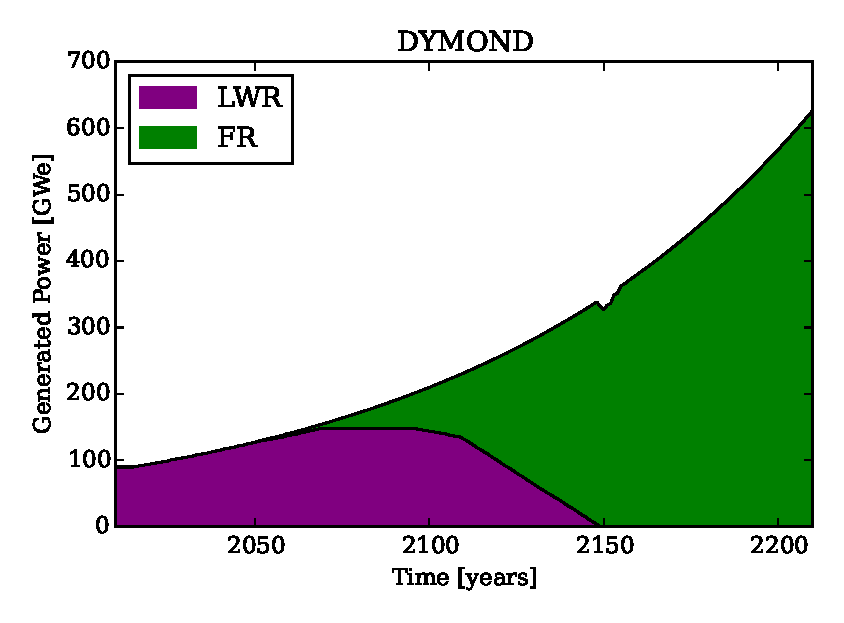
\includegraphics[width=0.45\textwidth]{gwe-dymond.eps}
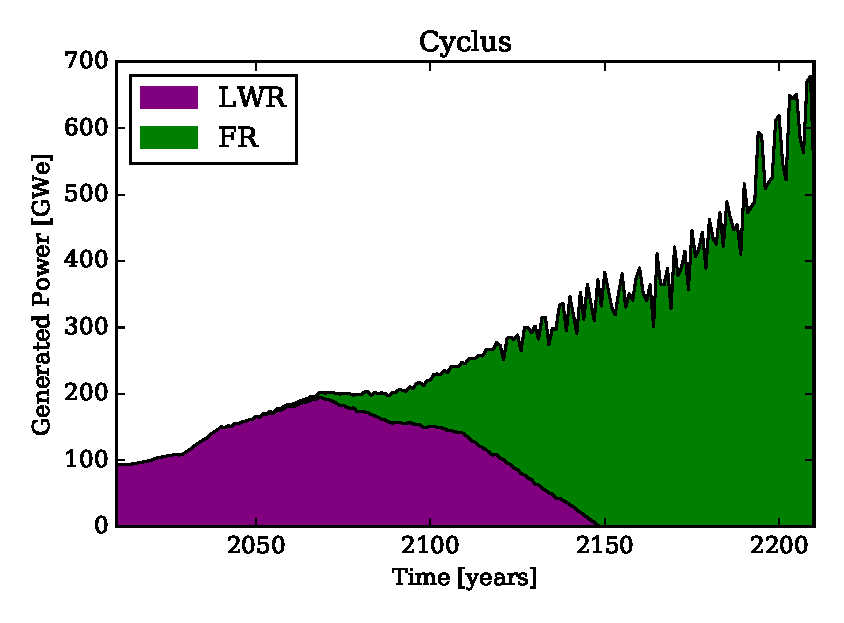
\includegraphics[width=0.45\textwidth]{gwe-cyclus.eps}
\caption{The generated power in [GWe] as a function of time for the DYMOND and 
Cyclus simulators for both LWRs and FRs.}
\label{gwe-simulators}
\end{figure}

The demonstration here will use the generated power from LWRs and FRs in 
a transition that covers 200 years. The simulation should start with
90 GWe generated solely by LWRs and meet a 1\% annual growth in demand over the 
lifetime of the simulation. Figure \ref{gwe-simulators} shows the component time 
series curves for both DYMOND and Cyclus. 

The difference between the LWR curves in Figure \ref{gwe-simulators} stem 
partially from how the simulators choose to implement the initial conditions.
DYMOND uses an initial condition that 
begins with a fleet that produces 90 GWe in 2010 and whose reactors are 
decommissioned on a staggered schedule. The Cyclus simulation, on the other 
hand, begins the simulation in 1960 and deploys two reactors per year for
the first fifty years. This yields 100 LWRs in 2010 that have a refueling 
schedule and capacity factor such that 90 GWe of power is generated. Since
Cyclus is agent-based, these reactors then decommission themselves naturally
given their 60 year lifespan. New reactors are subsequently deployed after
2010.

The difference between the FR curves in Figure \ref{gwe-simulators} come
from modeling differences in the simulators themselves. DYMOND does not 
restrict FRs from operating once they are deployed even if fresh fuel is not 
immediately available. Cyclus, however, does model fuel shortages and 
reactors will sit idle until valid fresh fuel becomes available. Furthermore, 
in the Cyclus simulation here (i.e. not a limitation of Cyclus itself), 
all reactors are deployed only in January of each the year.
This leads to the oscillations seen at later times (2135+) because all 
FRs that begin on the same time step will shut down for their first
refueling at the same time, all of those that obtain fuel will go down for 
their second refueling at the same time, and so on. As more FRs are deployed, 
this effect becomes more pronounced. DYMOND, on the other hand, models a 
scalar capcity factor and does not produce these oscillations.

The next section describes how to
construct Gaussian process models from the data set presented above.

\clearpage
